\documentclass[]{article}
\usepackage{mathtools}
\usepackage[pdftex]{graphicx}	
\usepackage{amsmath,amsfonts,amsthm}	
\usepackage{tikz}
\usetikzlibrary{chains, positioning}
\newtheorem{theorem}{Theorem}[section]
\newtheorem{lemma}[theorem]{Lemma}
\newtheorem{proposition}[theorem]{Proposition}
\newtheorem{corollary}[theorem]{Corollary}
\usepackage{sidecap}
\theoremstyle{definition}
\newtheorem{definition}{Definition}[section]

\usetikzlibrary{calc,arrows}

%opening
\title{Activation functions}
\author{Rafa\"l Skrzypiec}
\date{}
\begin{document}
\maketitle

\section{Activation functions}

There are many possible choices for the non-linear activation functions in a multilayered network... biology 
czemu non-linear?
różne funkcje w zależności od zastosowań, ReLU, Sigmiod, TanH, Heavyside 
\begin{figure}[h!]
	\centering
	\includegraphics[width=\linewidth]{activations14_12}
	\caption{COO}
\end{figure}



\subsection{Sigmoid}
-nieliniowa
-dobrze odwzorowuje liniowe zaleznosci dla niewielkich wag
-moze byc funkcją schodkową dla dużej wartosci sumy
-prosta pochodna

\begin{figure}[h!]
	\centering
	\includegraphics[width=\linewidth]{sigmoid14_8}
	\caption{Example of sigmoidal function - sigmoid function, $\sigma(x) = \frac{1}{1+e^{-x}}$}
\end{figure} 
narysować jeszcze tanh, związek z sigmoidą, jeden obrazek z kilkoma funkcjami aktywacji

\newpage

\subsection{Probabilistic interpretation of sigmoid}


The application of sigmoid as an activation function arises naturally as the form of the posterior probability distribution in Bayesian treatment of two-class classification problem.
%
Let us consider a single-layer network and the concept of a discriminant function $y(x)$, such that the vector $x$ is assigned to class $C_1$ if $y(x) > 0$ and to class $C_2$ if $y(x) < 0$.
\\

In the simplest, linear form, discriminant function can be written as:
%
\begin{equation}
y(x) = w^\mathsf{T} x + b_0.
\end{equation}
%
We should refer to d-dimensional vector $w$ as the weight vector and the parameter $b_0$ as the bias.
There are several ways to generalize such functions, here we consider a function $g(\cdot)$ called activation function that acts on a aforementioned linear sum, and gives a discrimination function of the form
%
\begin{equation}
y = g\left(w^\mathsf{T} x + b_0 \right)
\end{equation}
%
\def\layersep{2.5cm}

	\begin{SCfigure}
		\centering

	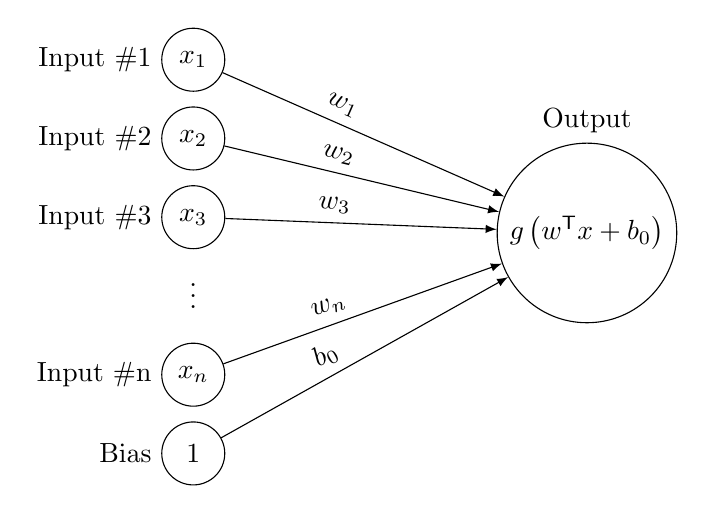
\begin{tikzpicture}
	[   cnode/.style={draw=black,draw=black,fill=#1,minimum width=8mm,circle},
	]
	\tikzset{normal arrow/.style={draw,-latex}}
	\node[cnode=white,label=90:Output] (s) at (5,-3.2) {$ g\left(w^\mathsf{T} x + b_0 \right)$};
	\node at (0,-3.9) {$\vdots$};
	
	\node[cnode=white,label=180:Bias] (x-5) at (0,-6) {1};
	
	\foreach \x in {1,...,4}
	{
		\pgfmathparse{\x<4 ? \x : "n"}	   
		\ifnum \x = 4
		\node[cnode=white,label=180:Input \#n] (x-\x) at (0,{-1*\x-div(\x,4)}) {$x_{n}$};
		
		\else
		
		\node[cnode=white,label=180:Input \#\pgfmathresult] (x-\x) at (0,{-1*\x-div(\x,4)}) {$x_{\x}$};
		\fi
		\path[normal arrow] (x-\x) -- node[above,sloped,pos=0.4] {$w_{\pgfmathresult}$} (s);
	}
	\path[normal arrow] (x-5) -- node[above,sloped,pos=0.4] {$b_0$} (s);	
	\end{tikzpicture}
	\caption{ Representation of discriminant function $y(x)$ as a neural network diagram, having $n$ inputs, bias term and one output.  }
	\end{SCfigure}

%
Assumption that probability distribution functions of data given the class $C_k$ are given by Gaussian distributions with equal covariance matrices $ \Sigma_1 = \Sigma_2 = \Sigma$ gives:
%
\begin{equation}
p(x|C_k) = \frac{1}{\left(2 \pi\right)^{\frac{d}{2}} \left| \Sigma \right|^{\frac{1}{2}}} \exp \left[ -\frac{1}{2} \left(x - \mu_k\right)^\mathsf{T} \Sigma^{-1} \left(x - \mu_k \right) \right].
\end{equation}
%
The posterior probability of class $C_1$ can be written using Bayes' theorem:
%
\begin{eqnarray}
	p(C_1 | x) &=& \frac{p(x|C_1) p(C_1)}{ p(x|C_1) p(C_1) + p(x|C_2)p(C_2)} \nonumber\\
			   &=& \frac{1}{1 + \frac{p(x|C_2)p(C_2)}{p(x|C_1)p(C_1)}} \nonumber\\ 
			   &=& \frac{1}{1 + \exp(-a)},
\end{eqnarray}
%
where
%
\begin{eqnarray}
 a &=& \ln \frac{p(x|C_1)p(C_1)}{p(x|C_2)p(C_2)} \nonumber \\
 &=& \left( \mu_1 - \mu_2 \right)^{\mathsf{T}} \Sigma^{-1} x  - \frac{1}{2} \mu_1^\mathsf{T}\mu_1 + \frac{1}{2} \mu_2^\mathsf{T} \Sigma^{-1} \mu_2 + \ln \frac{p(C_1)}{p(C_2)},
\end{eqnarray}
%
hence
%
\begin{subequations}
	\begin{align}
		w &= \Sigma^{-1} \left(\mu_1 - \mu_2\right)\\
		b_0 &= - \frac{1}{2} \mu_1^\mathsf{T}\mu_1 + \frac{1}{2} \mu_2^\mathsf{T} \Sigma^{-1} \mu_2 + \ln \frac{p(C_1)}{p(C_2)}
	\end{align}
\end{subequations}

Thus the network output is given by a sigmoid activation function acting on a weighted linear combination of inputs. This reasoning can be generalized to multi-layered network. Then outputs of each hidden neuron with logistic sigmoid activation function can be interpreted as probabilities of the presence of corresponding attribute conditioned by the inputs. 




\end{document}
